\section{Introduction}
Over the past decade, software development has undergone significant evolution, driven by advances in mobile technology, cloud infrastructure, and real-time data processing. These innovations have enabled the creation of intelligent, responsive, and highly scalable applications that address real-world needs across various domains

In this context, the design and implementation of our student attendance tracking system is a practical example of applying modern technologies to solve persistent challenges in the academic environment. The focus of this project was to build a reliable and secure solution that leverages cross-platform mobile development, QR code functionality, and real-time data handling to ensure accurate and efficient attendance monitoring.

In this chapter, we present the technical implementation of the student attendance tracking application based on QR code technology. This chapter highlights the practical realization of the system, detailing the tools, technologies and a presentation of our application different interfaces.

\section{Technical Implementation}

\subsection{Technology Stack}
The project is built using a modern and robust technology stack that ensures scalability, real-time capabilities, and a smooth user experience:

\subsubsection{Flutter Framework}
Flutter is an open-source UI software development toolkit created by Google. It serves as the primary framework for building the cross-platform application in this project. Flutter enables developers to write a single codebase that can be compiled to run on Android, iOS, web, desktop, and embedded platforms, making it highly versatile and efficient for mobile app development~\cite{flutterDocs} .
It's main advantages are :
\begin{itemize}
    \item Cross-platform development capability for Android, iOS, and web platforms
    \item Rich set of customizable widgets for building responsive UIs
    \item Hot reload feature for rapid development
    \item High performance with native compilation
    \item Version: SDK $\geq$ 3.1.3
\end{itemize}

\subsubsection{Supabase Backend}

Supabase (version 2.6.3) is utilized as the backend solution for this application. It is an open-source Backend-as-a-Service (BaaS) platform that provides developers with scalable, real-time backend functionality built on top of PostgreSQL. Supabase offers a robust alternative to proprietary cloud services, enabling fast development of secure and efficient applications \cite{supabaseDocs}.

The main features leveraged in this project include:
\begin{itemize}
    \item Real-time database capabilities
    \item Built-in authentication system
    \item Powerful PostgreSQL database
    \item Real-time subscriptions for live updates
    \item Secure API access
\end{itemize}


\subsubsection{Key Dependencies}
The application leverages several essential packages:
\begin{itemize}
    \item \texttt{flutter\_riverpod} (v2.4.9): State management solution
    \item \texttt{qr\_flutter} (v4.1.0): QR code generation
    \item \texttt{qr\_code\_scanner\_plus} (v2.0.10): QR code scanning
    \item \texttt{flutter\_speed\_dial} (v7.0.0): Advanced floating action button
    \item \texttt{fl\_chart} (v0.66.2): Data visualization
    \item \texttt{web\_socket\_channel} (v2.4.0): Real-time communication
\end{itemize}

\subsection{Hardware and Software Requirements}

\subsubsection{Hardware Requirements}
\begin{itemize}
    \item Smartphone or tablet with camera capability for QR scanning
    \item Minimum 2GB RAM recommended
    \item At least 100MB of storage space
    \item Internet connectivity (WiFi or mobile data)
\end{itemize}

\subsubsection{Software Requirements}
\begin{itemize}
    \item Android: Android 5.0 (API level 21) or higher
    \item iOS: iOS 11.0 or higher
    \item Web browsers: Latest versions of Chrome, Firefox, Safari, or Edge
    \item Internet connection for real-time features
\end{itemize}

%\clearpage
\subsection{Implementation Details}

\subsubsection{System Architecture}
The application follows a clean architecture pattern with clear separation of concerns:
\begin{itemize}
    \item UI Layer: Widgets and screens
    \item Business Logic: Providers and services
    \item Data Layer: Models and repositories
    \item Infrastructure: API clients and local storage
\end{itemize}

\subsubsection{Key Features and Functionality}

\needspace{4\baselineskip}
\subsection{Authentication System}\nopagebreak[4]
\begin{itemize}
    \item Secure user authentication via Supabase
    \item Role-based access control (Teacher/Student)
    \item Persistent session management
\end{itemize}

\needspace{4\baselineskip}
\subsection{QR Code Attendance System}\nopagebreak[4]
\begin{itemize}
    \item Dynamic QR code generation for sessions
    \item Real-time QR code scanning and validation
    \item Attendance tracking and verification
\end{itemize}

\needspace{4\baselineskip}
\subsection{Real-time Updates}\nopagebreak[4]
\begin{itemize}
    \item Live attendance tracking
    \item Instant status updates
    \item WebSocket-based notifications
\end{itemize}

\subsubsection{Interface Implementation}
The application features a responsive interface that adapts seamlessly between mobile and desktop views, providing an optimal user experience across different screen sizes. Each interface component is carefully designed to maintain functionality while adjusting its layout based on the available screen space.

\needspace{4\baselineskip}
\subsection{Home Dashboard}\nopagebreak[4]
\begin{figure}[H]
    \centering
    \begin{subfigure}[b]{0.35\textwidth}
        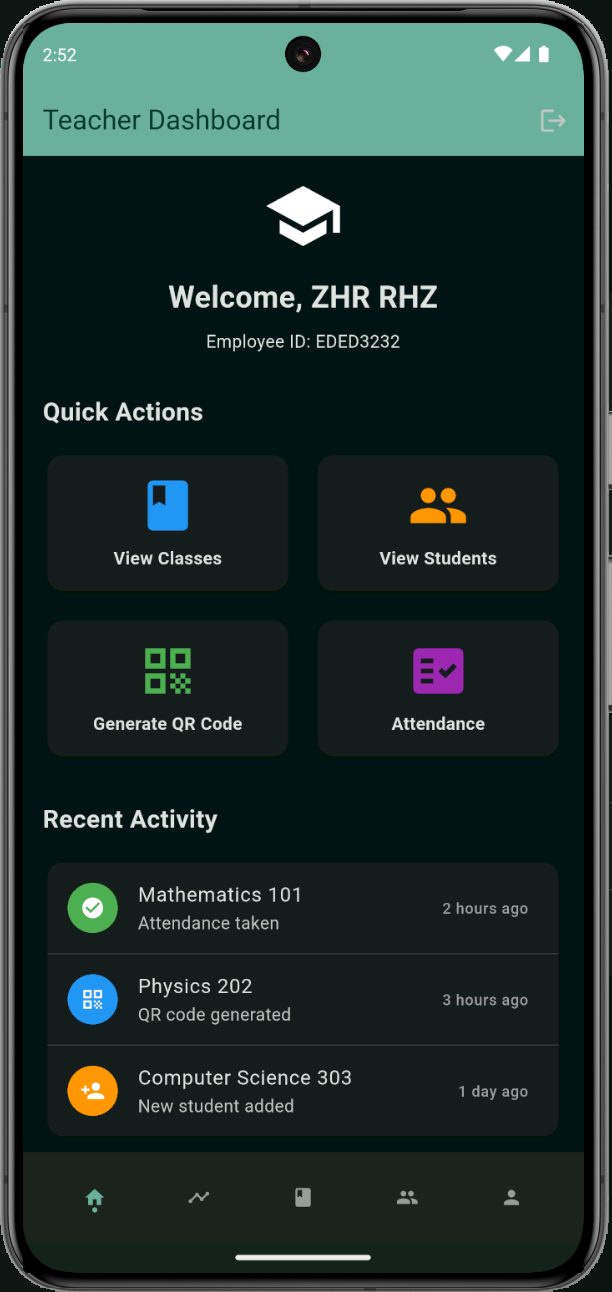
\includegraphics[width=\textwidth]{images/rachid/teacher-side-home.png}
        \caption{Mobile view showing quick access to key features and real-time attendance statistics}
    \end{subfigure}
    \hfill
    \begin{subfigure}[b]{0.35\textwidth}
        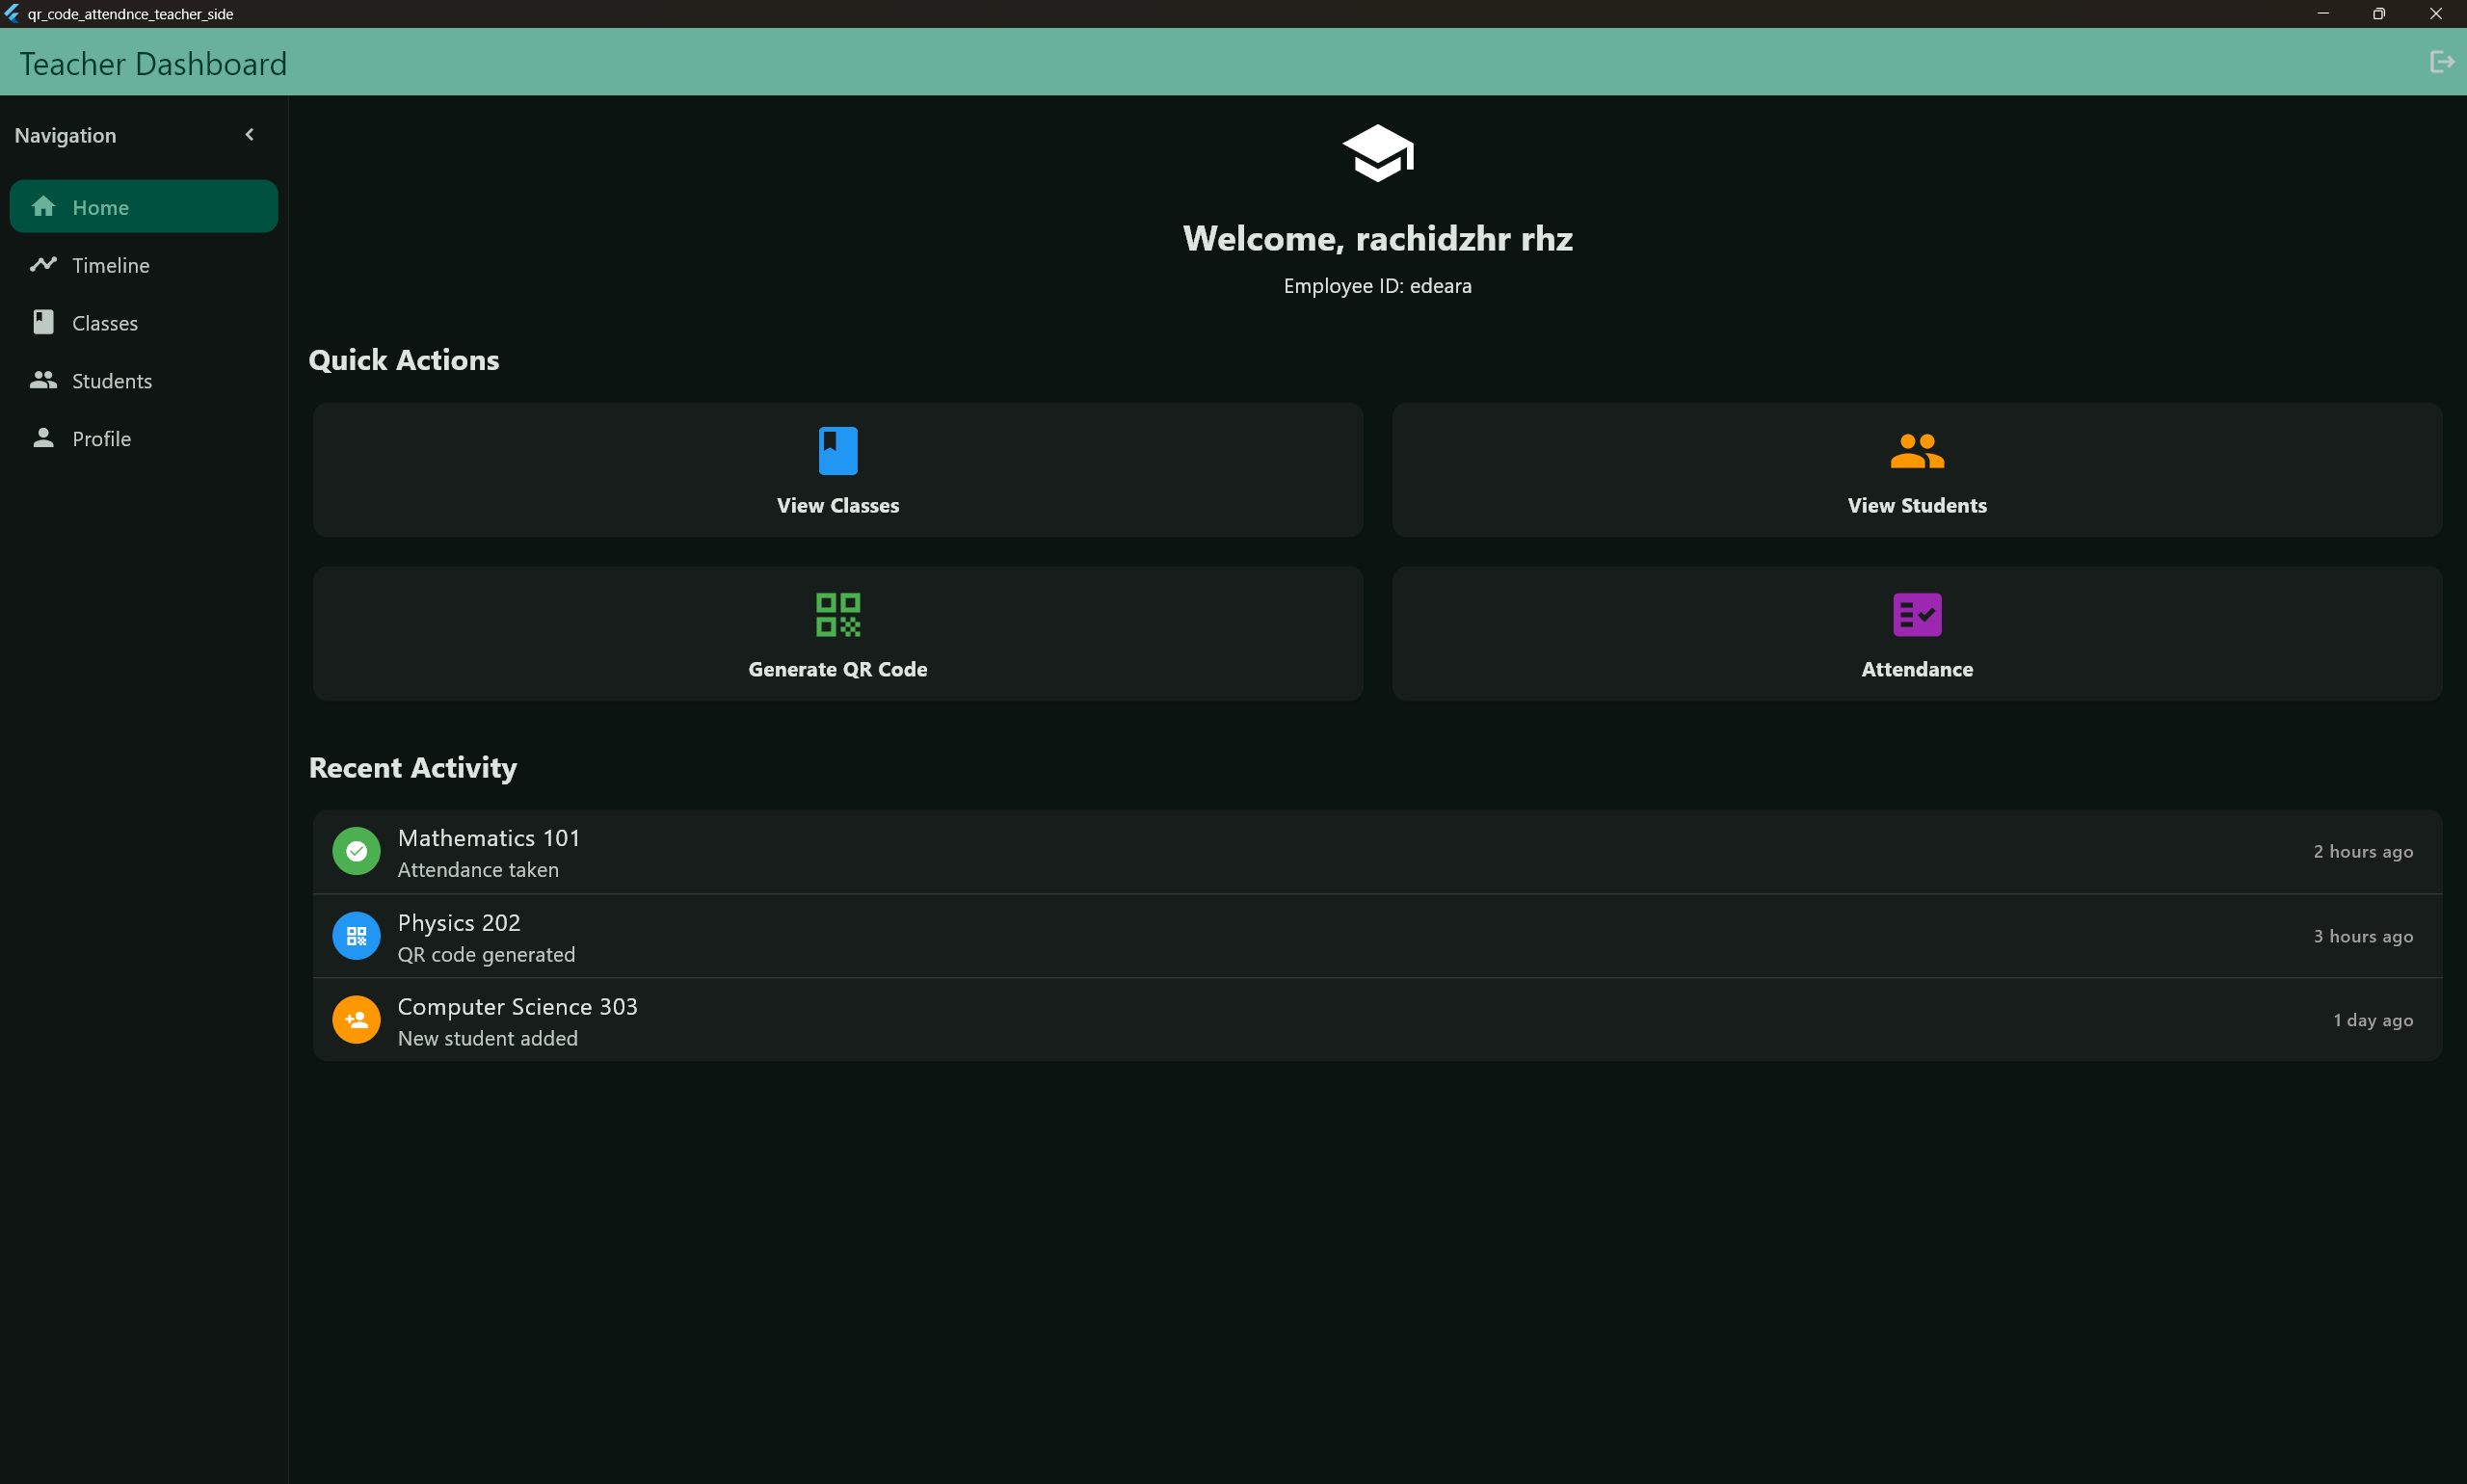
\includegraphics[width=\textwidth]{images/rachid/teacher-side-home-disktop.png}
        \caption{Desktop view with expanded navigation rail and detailed dashboard layout}
    \end{subfigure}
    \caption{Teacher's Home Dashboard Interface}
    \label{fig:home-interface}
\end{figure}

\needspace{4\baselineskip}
\subsection{Profile Management}\nopagebreak[4]
\begin{figure}[H]
    \centering
    \begin{subfigure}[b]{0.35\textwidth}
        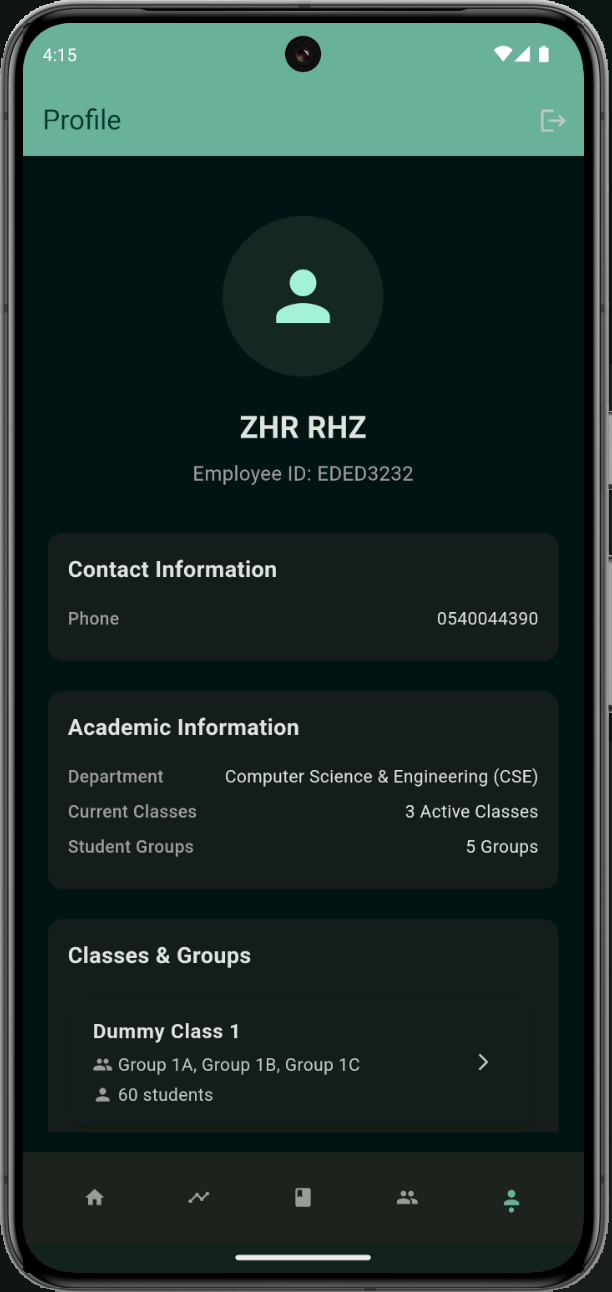
\includegraphics[width=\textwidth]{images/rachid/teacher-side-profile.png}
        \caption{Mobile view with compact profile information and quick actions}
    \end{subfigure}
    \hfill
    \begin{subfigure}[b]{0.35\textwidth}
        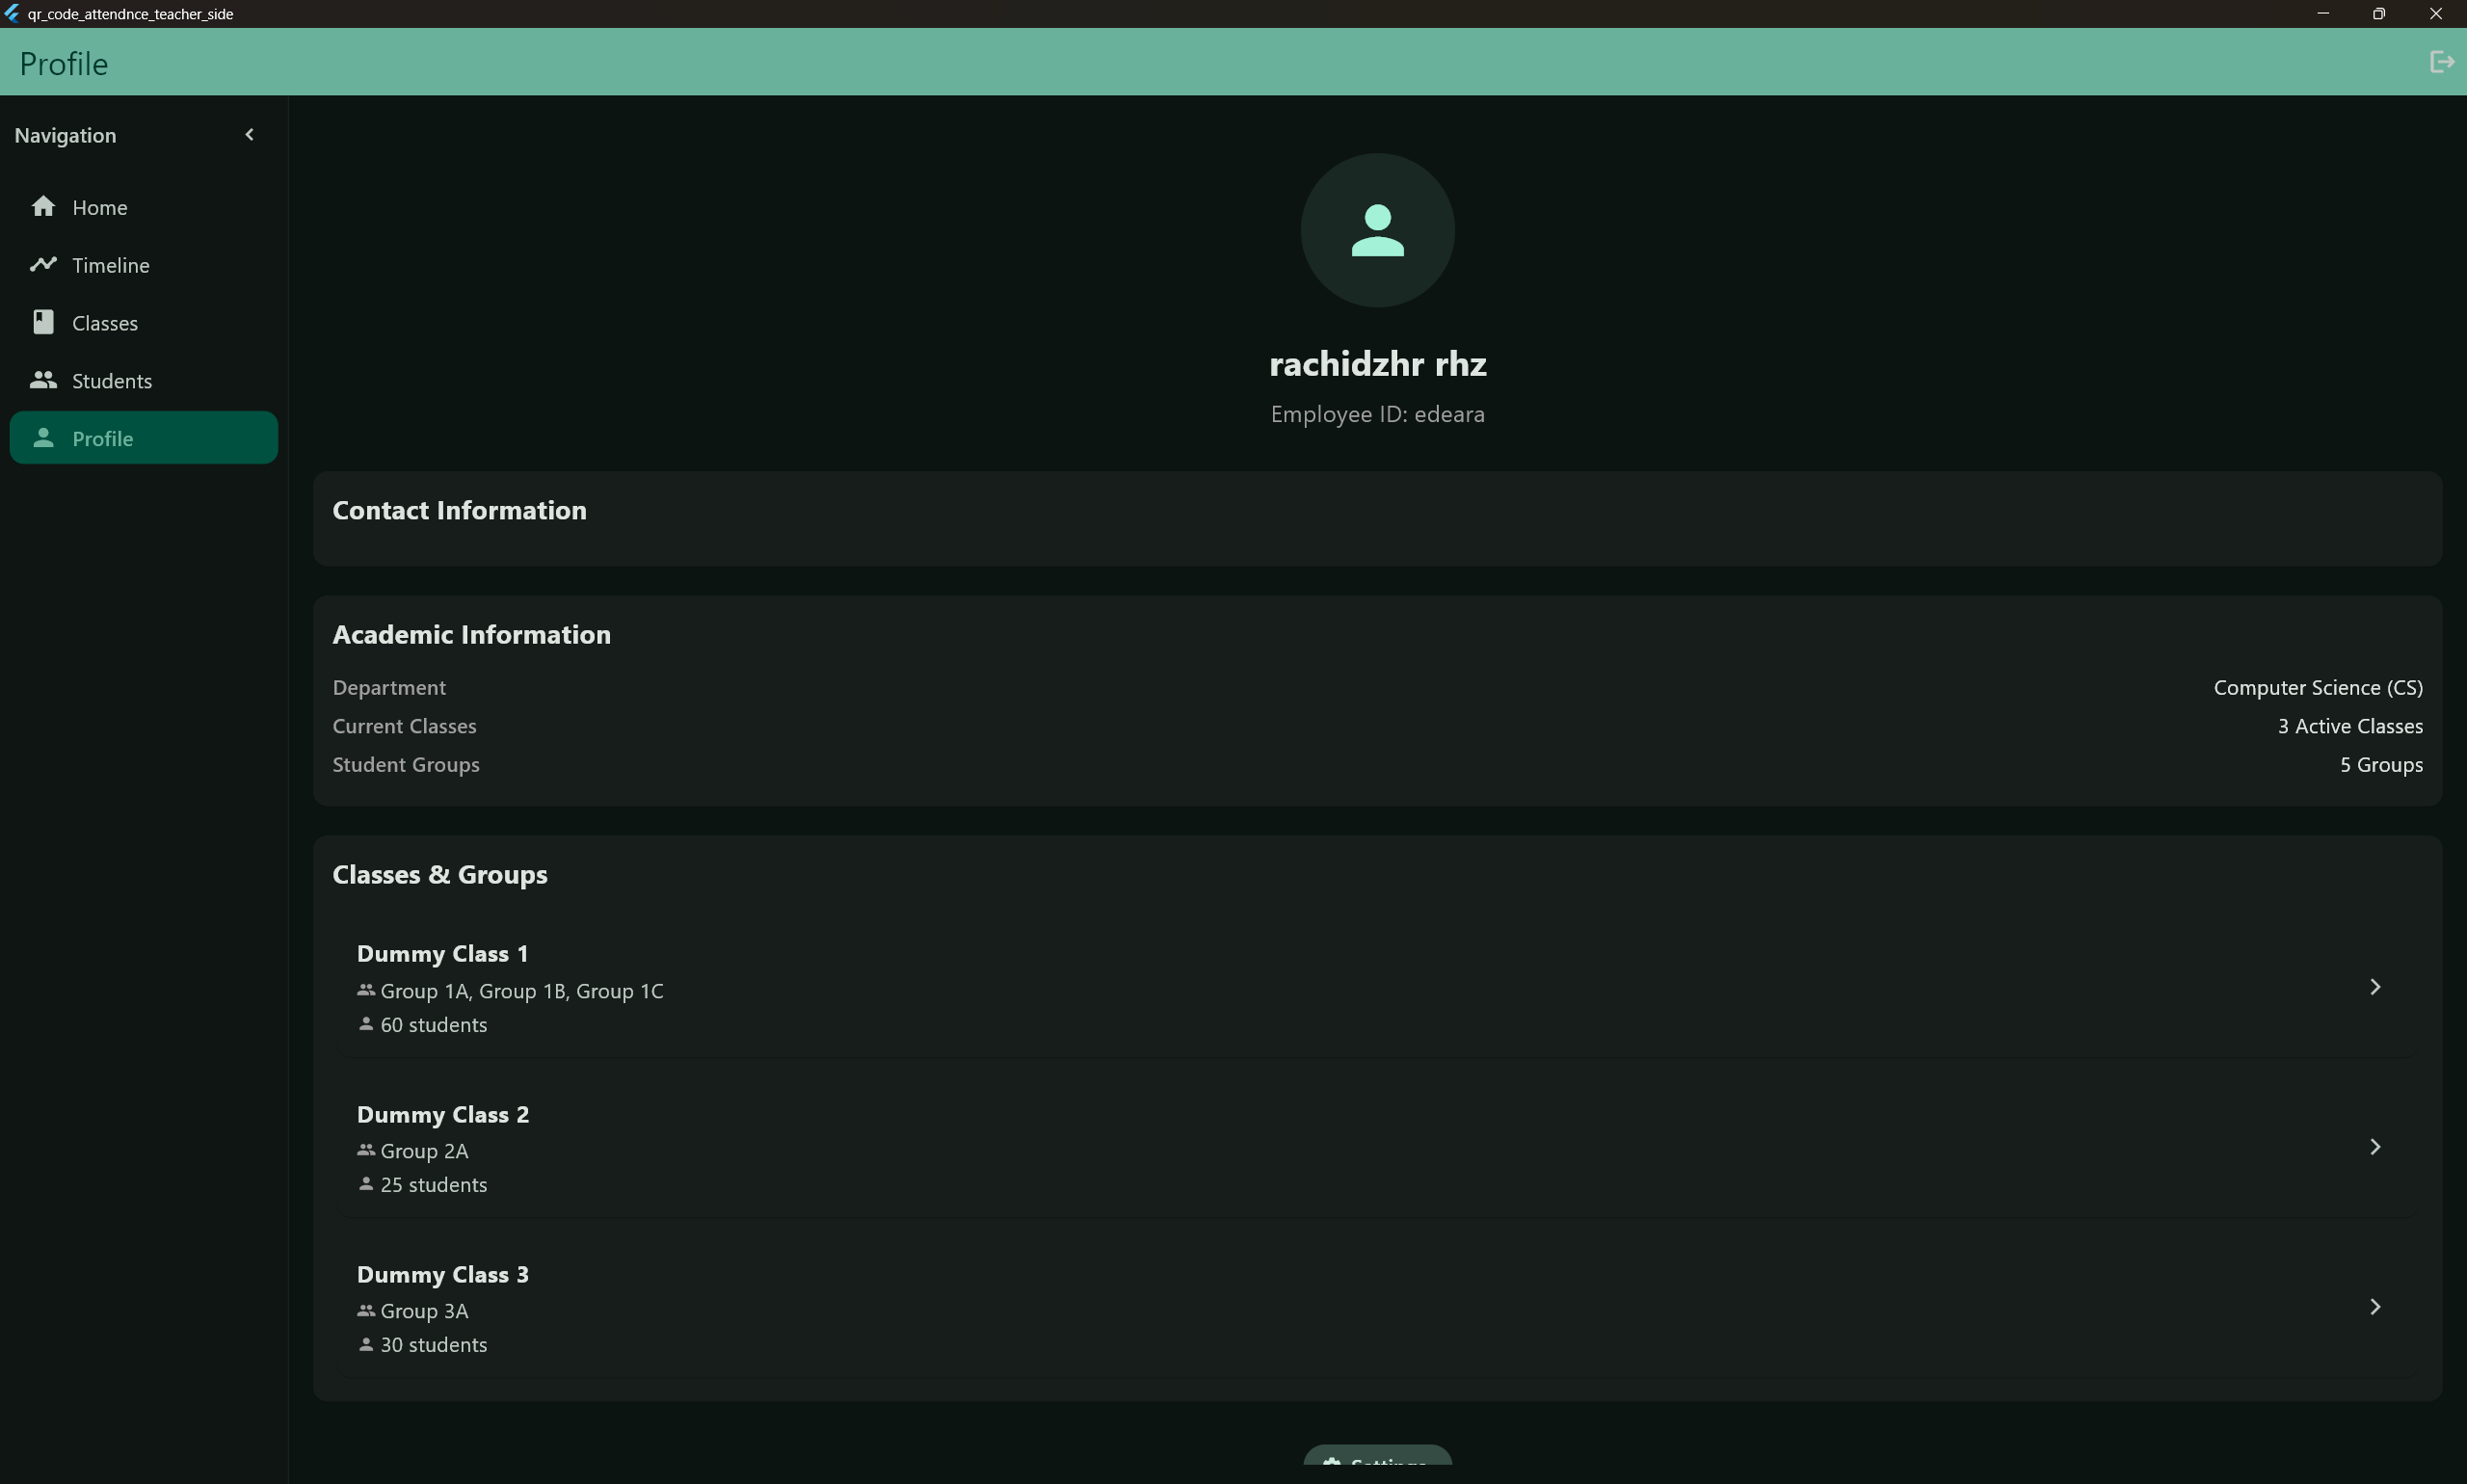
\includegraphics[width=\textwidth]{images/rachid/teacher-side-profile-disktop.png}
        \caption{Desktop view showing expanded profile details and statistics}
    \end{subfigure}
    \caption{Teacher Profile Management Interface}
    \label{fig:profile-interface}
\end{figure}

\needspace{4\baselineskip}
\subsection{Settings Interface}\nopagebreak[4]
\vspace{0.5cm}
\begin{figure}[H]
    \centering
    \begin{subfigure}[b]{0.35\textwidth}
        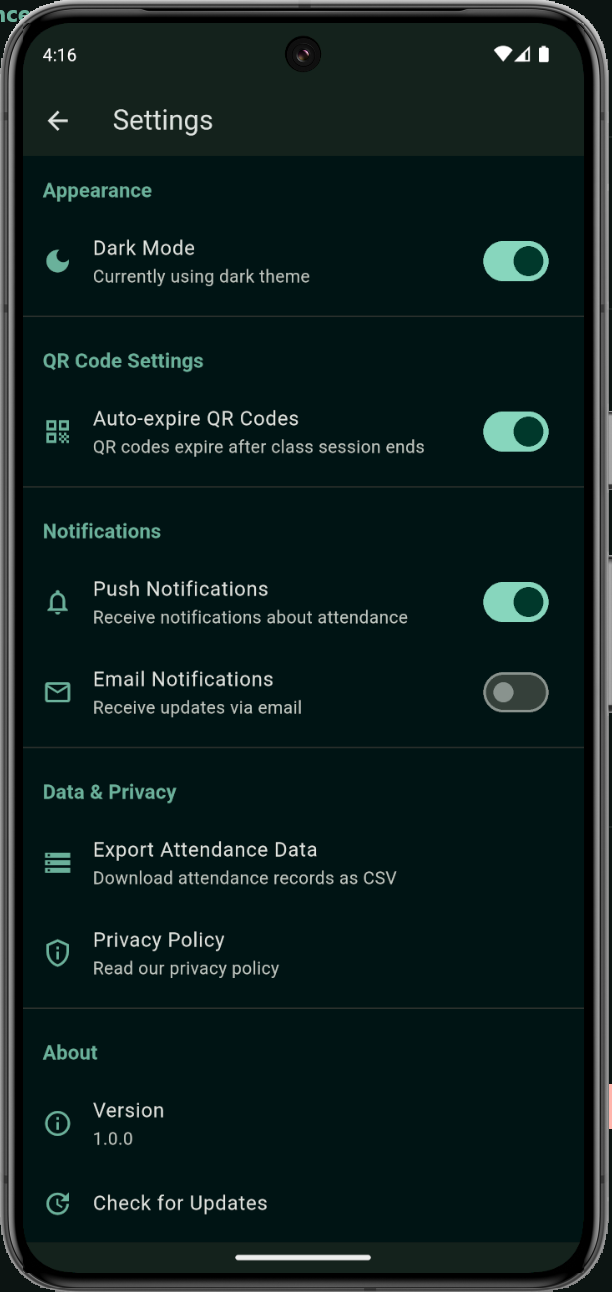
\includegraphics[width=\textwidth]{images/rachid/teacher-side-settings.png}
        \caption{Mobile settings view with scrollable preferences}
    \end{subfigure}
    \hfill
    \begin{subfigure}[b]{0.35\textwidth}
        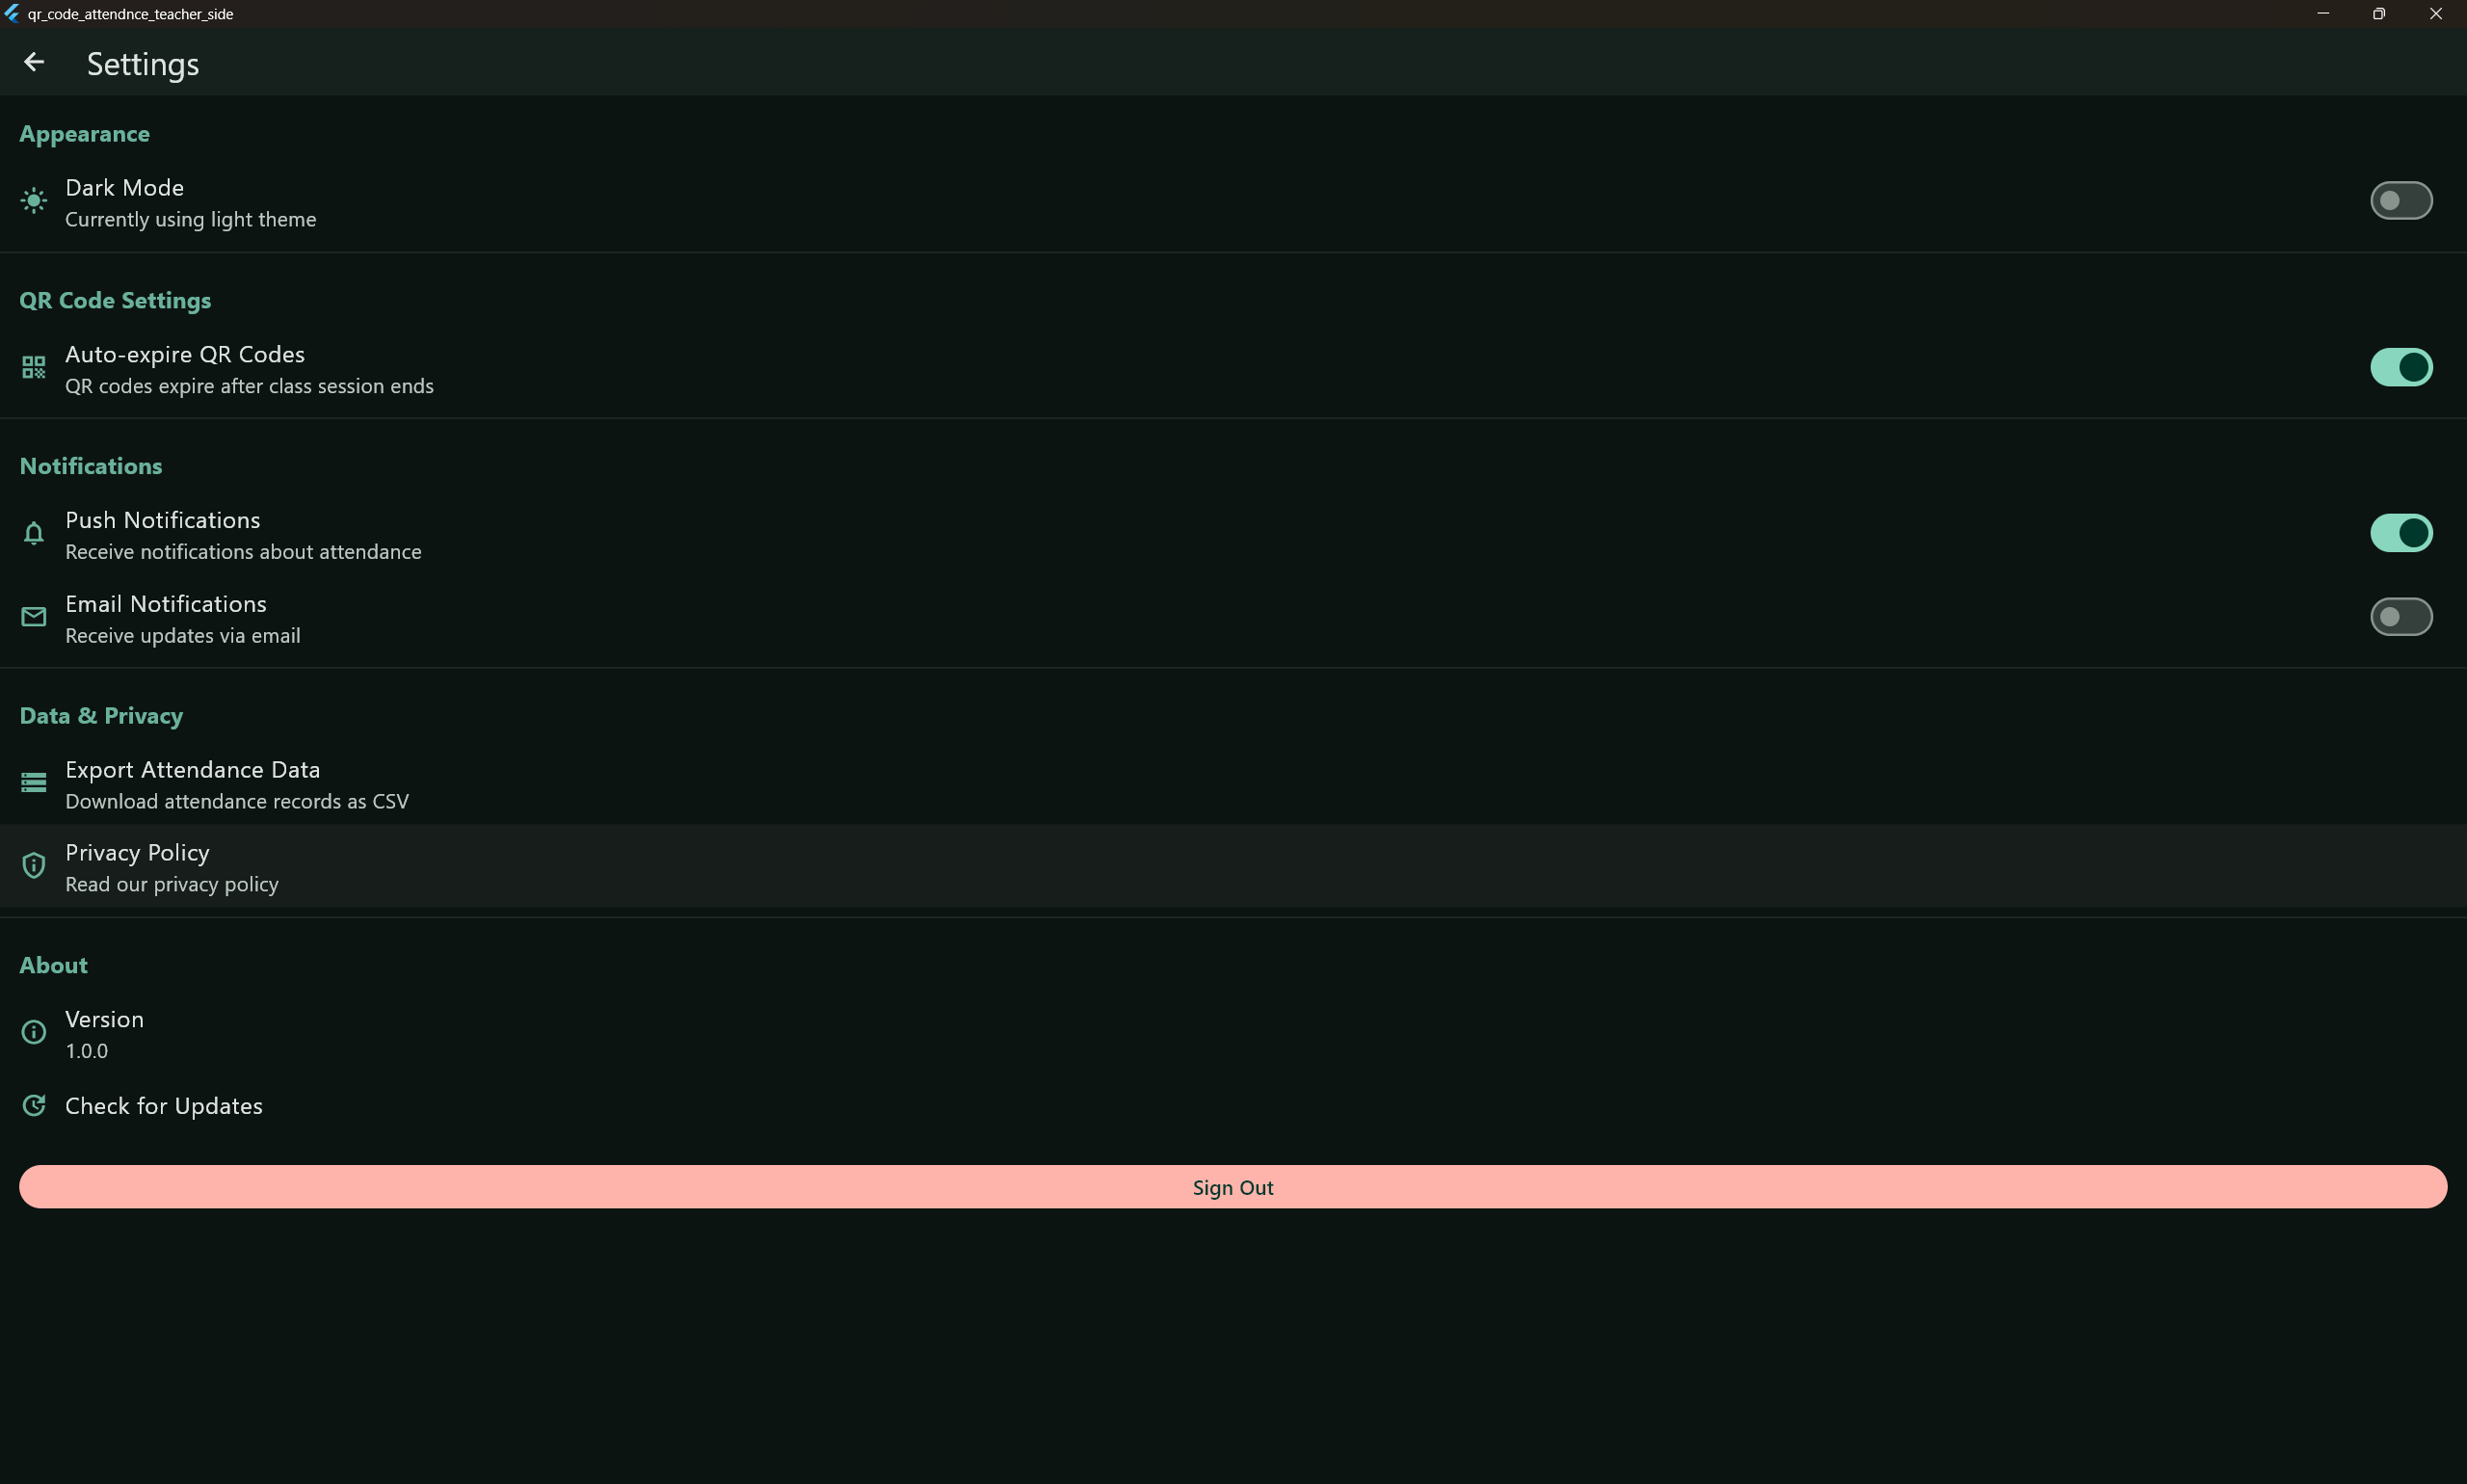
\includegraphics[width=\textwidth]{images/rachid/teacher-side-settings-desktop.png}
        \caption{Desktop settings panel with categorized options}
    \end{subfigure}
    \caption{Application Settings Interface}
    \label{fig:settings-interface}
\end{figure}

\needspace{4\baselineskip}
\subsection{Student Management}\nopagebreak[4]
\vspace{0.5cm}
\begin{figure}[H]
    \centering
    \begin{subfigure}[b]{0.35\textwidth}
        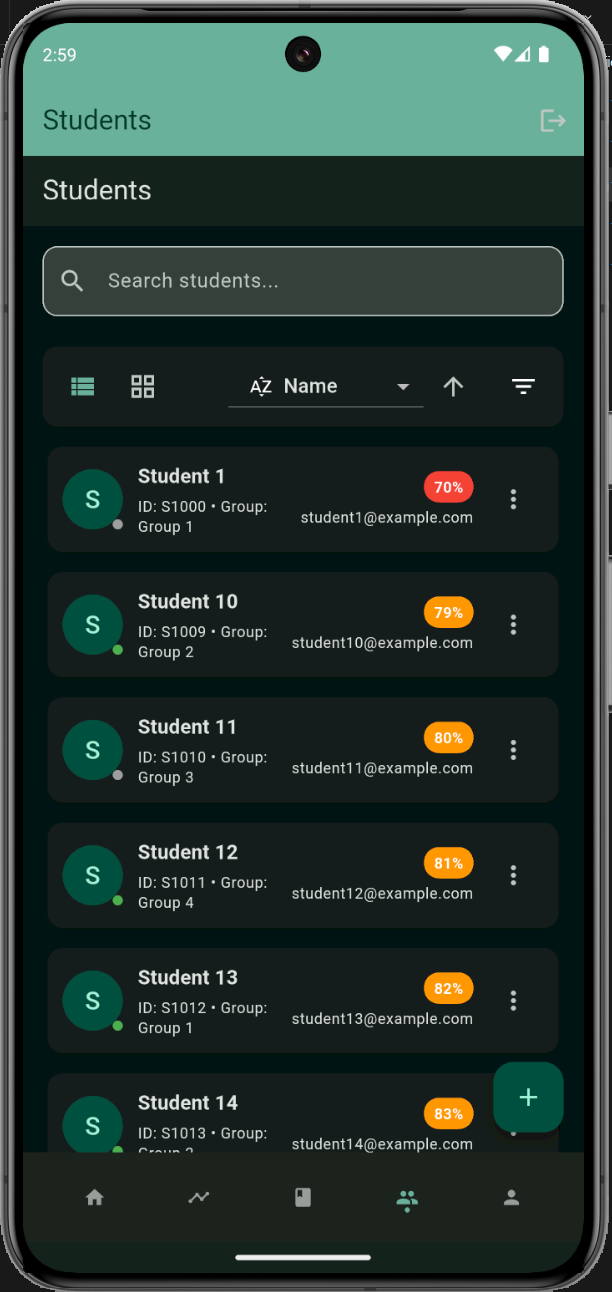
\includegraphics[width=\textwidth]{images/rachid/teacher-side-studentpage.png}
        \caption{Mobile student list with attendance status indicators}
    \end{subfigure}
    \hfill
    \begin{subfigure}[b]{0.35\textwidth}
        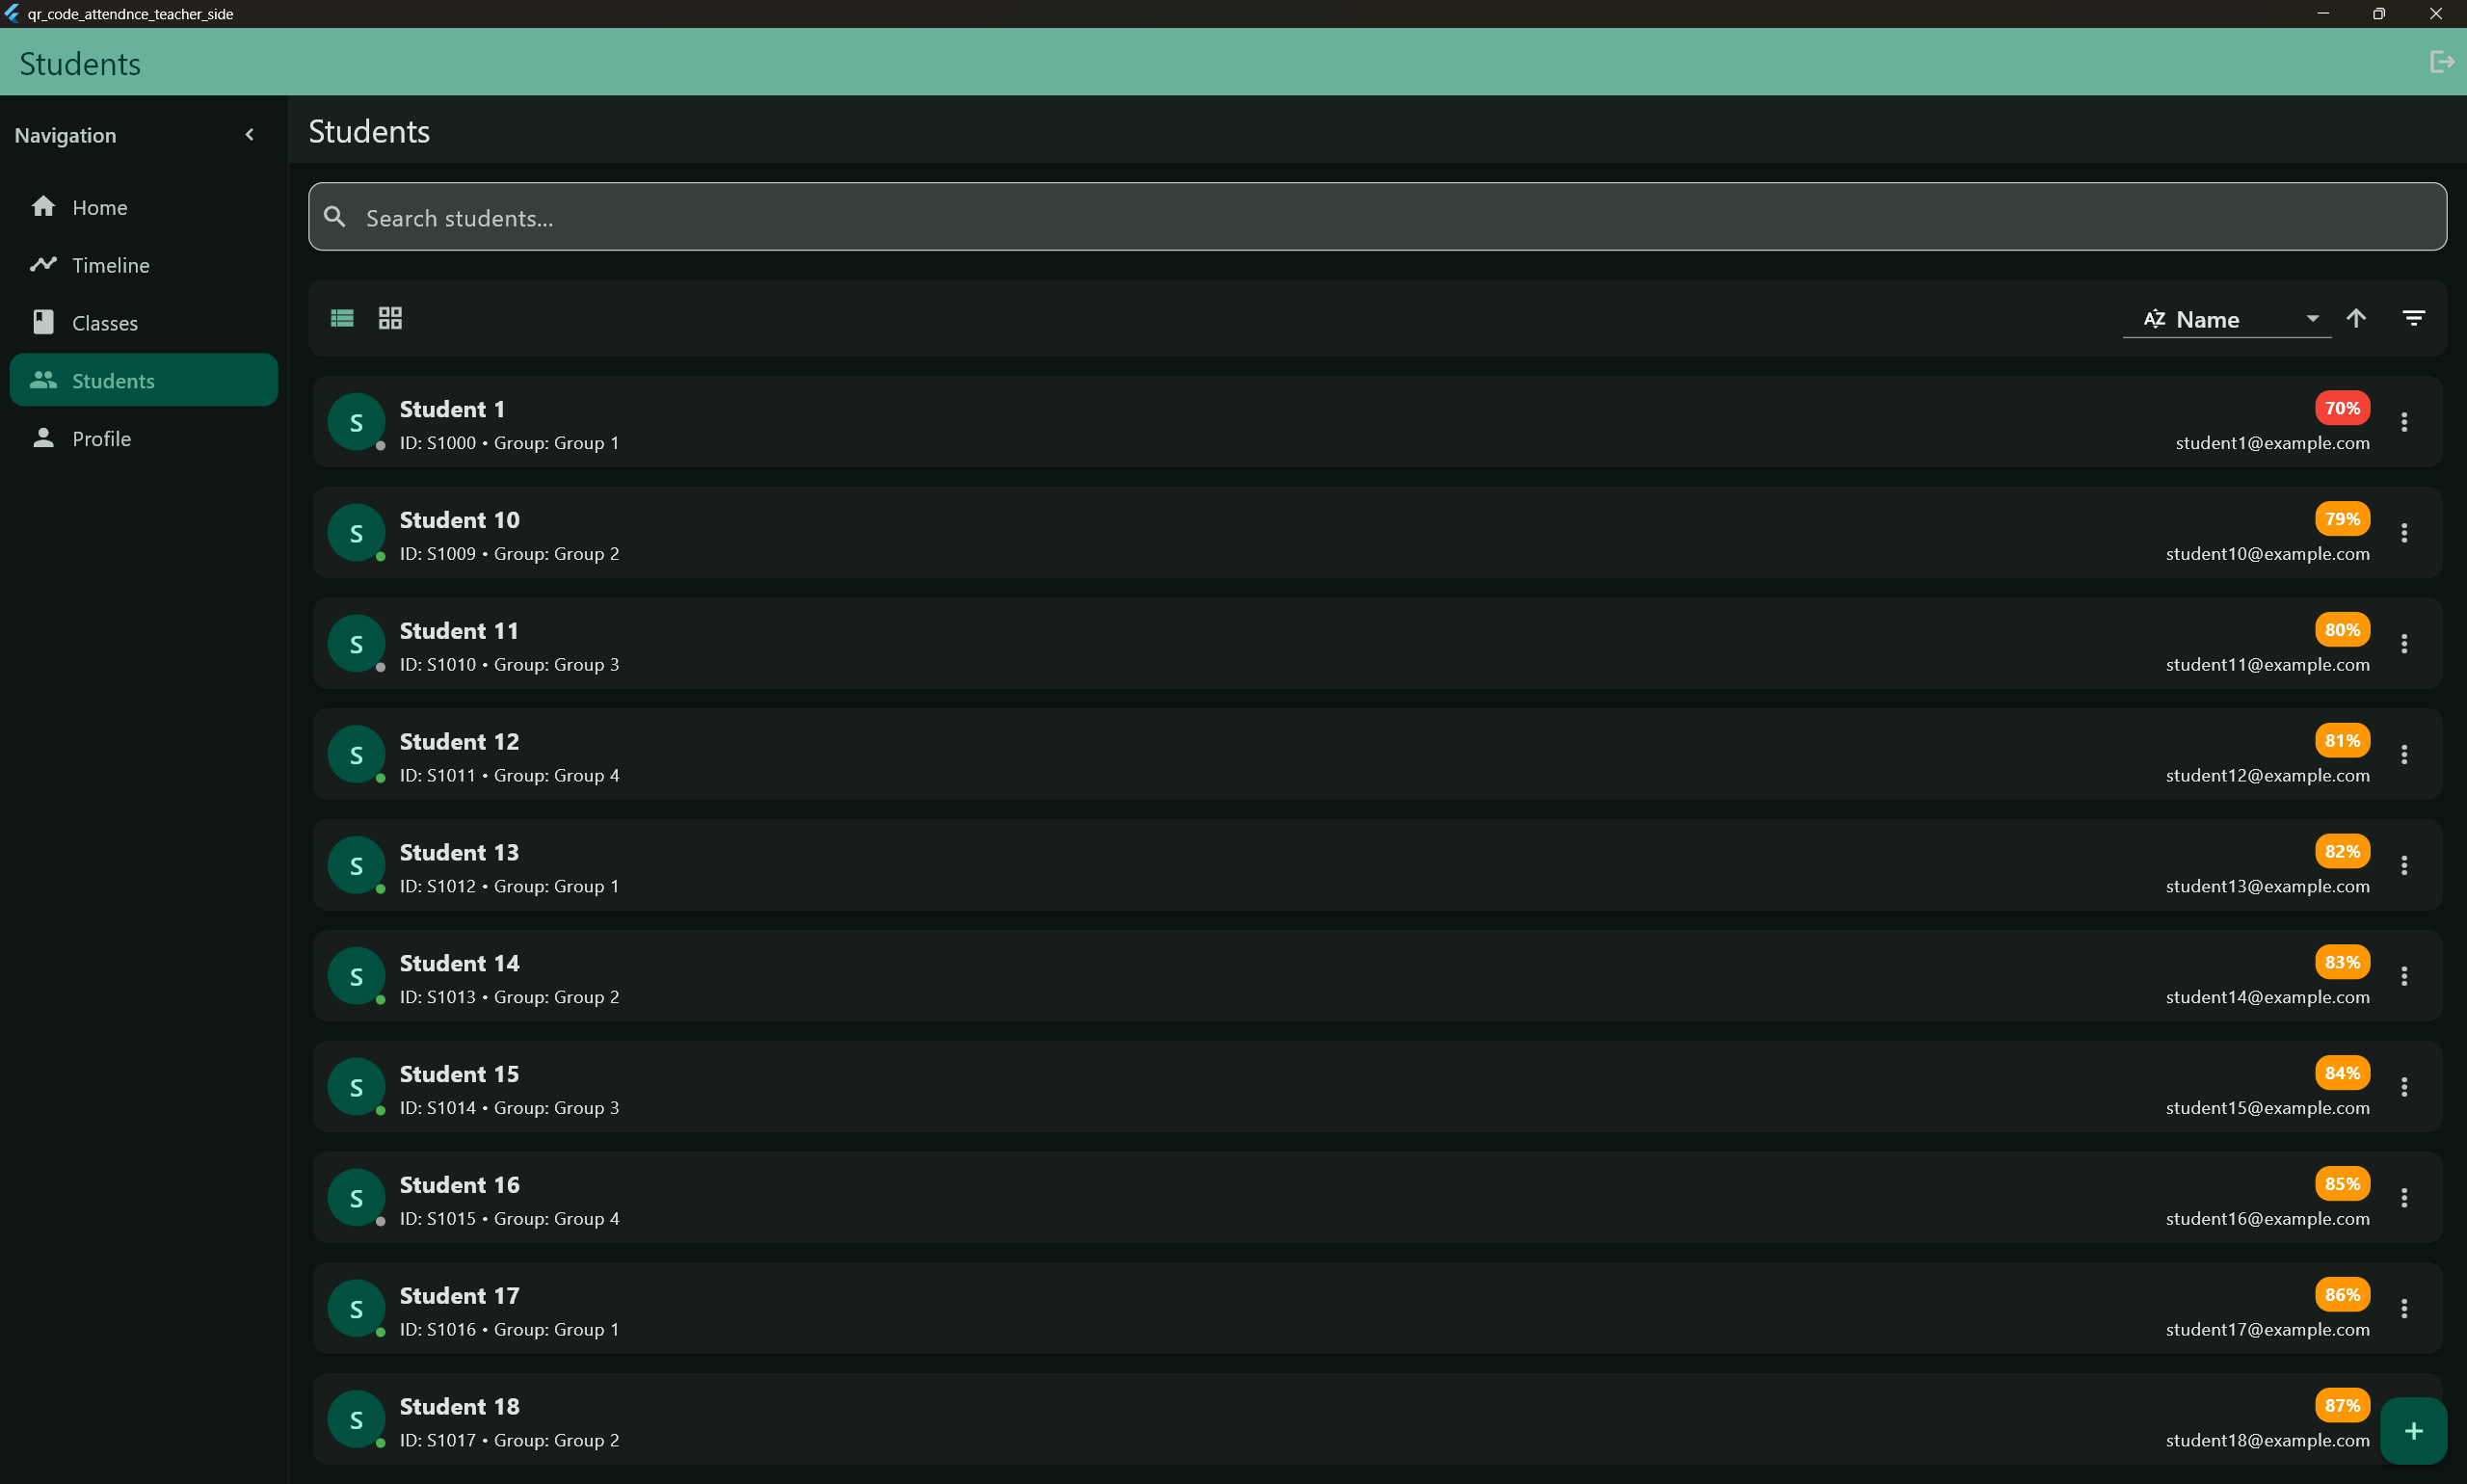
\includegraphics[width=\textwidth]{images/rachid/teacher-side-studentpage-desktop.png}
        \caption{Desktop view with enhanced student management tools}
    \end{subfigure}
    \caption{Student Management Interface}
    \label{fig:student-management}
\end{figure}

\needspace{4\baselineskip}
\subsection{Student Profile View}\nopagebreak[4]
\vspace{0.5cm}
\begin{figure}[H]
    \centering
    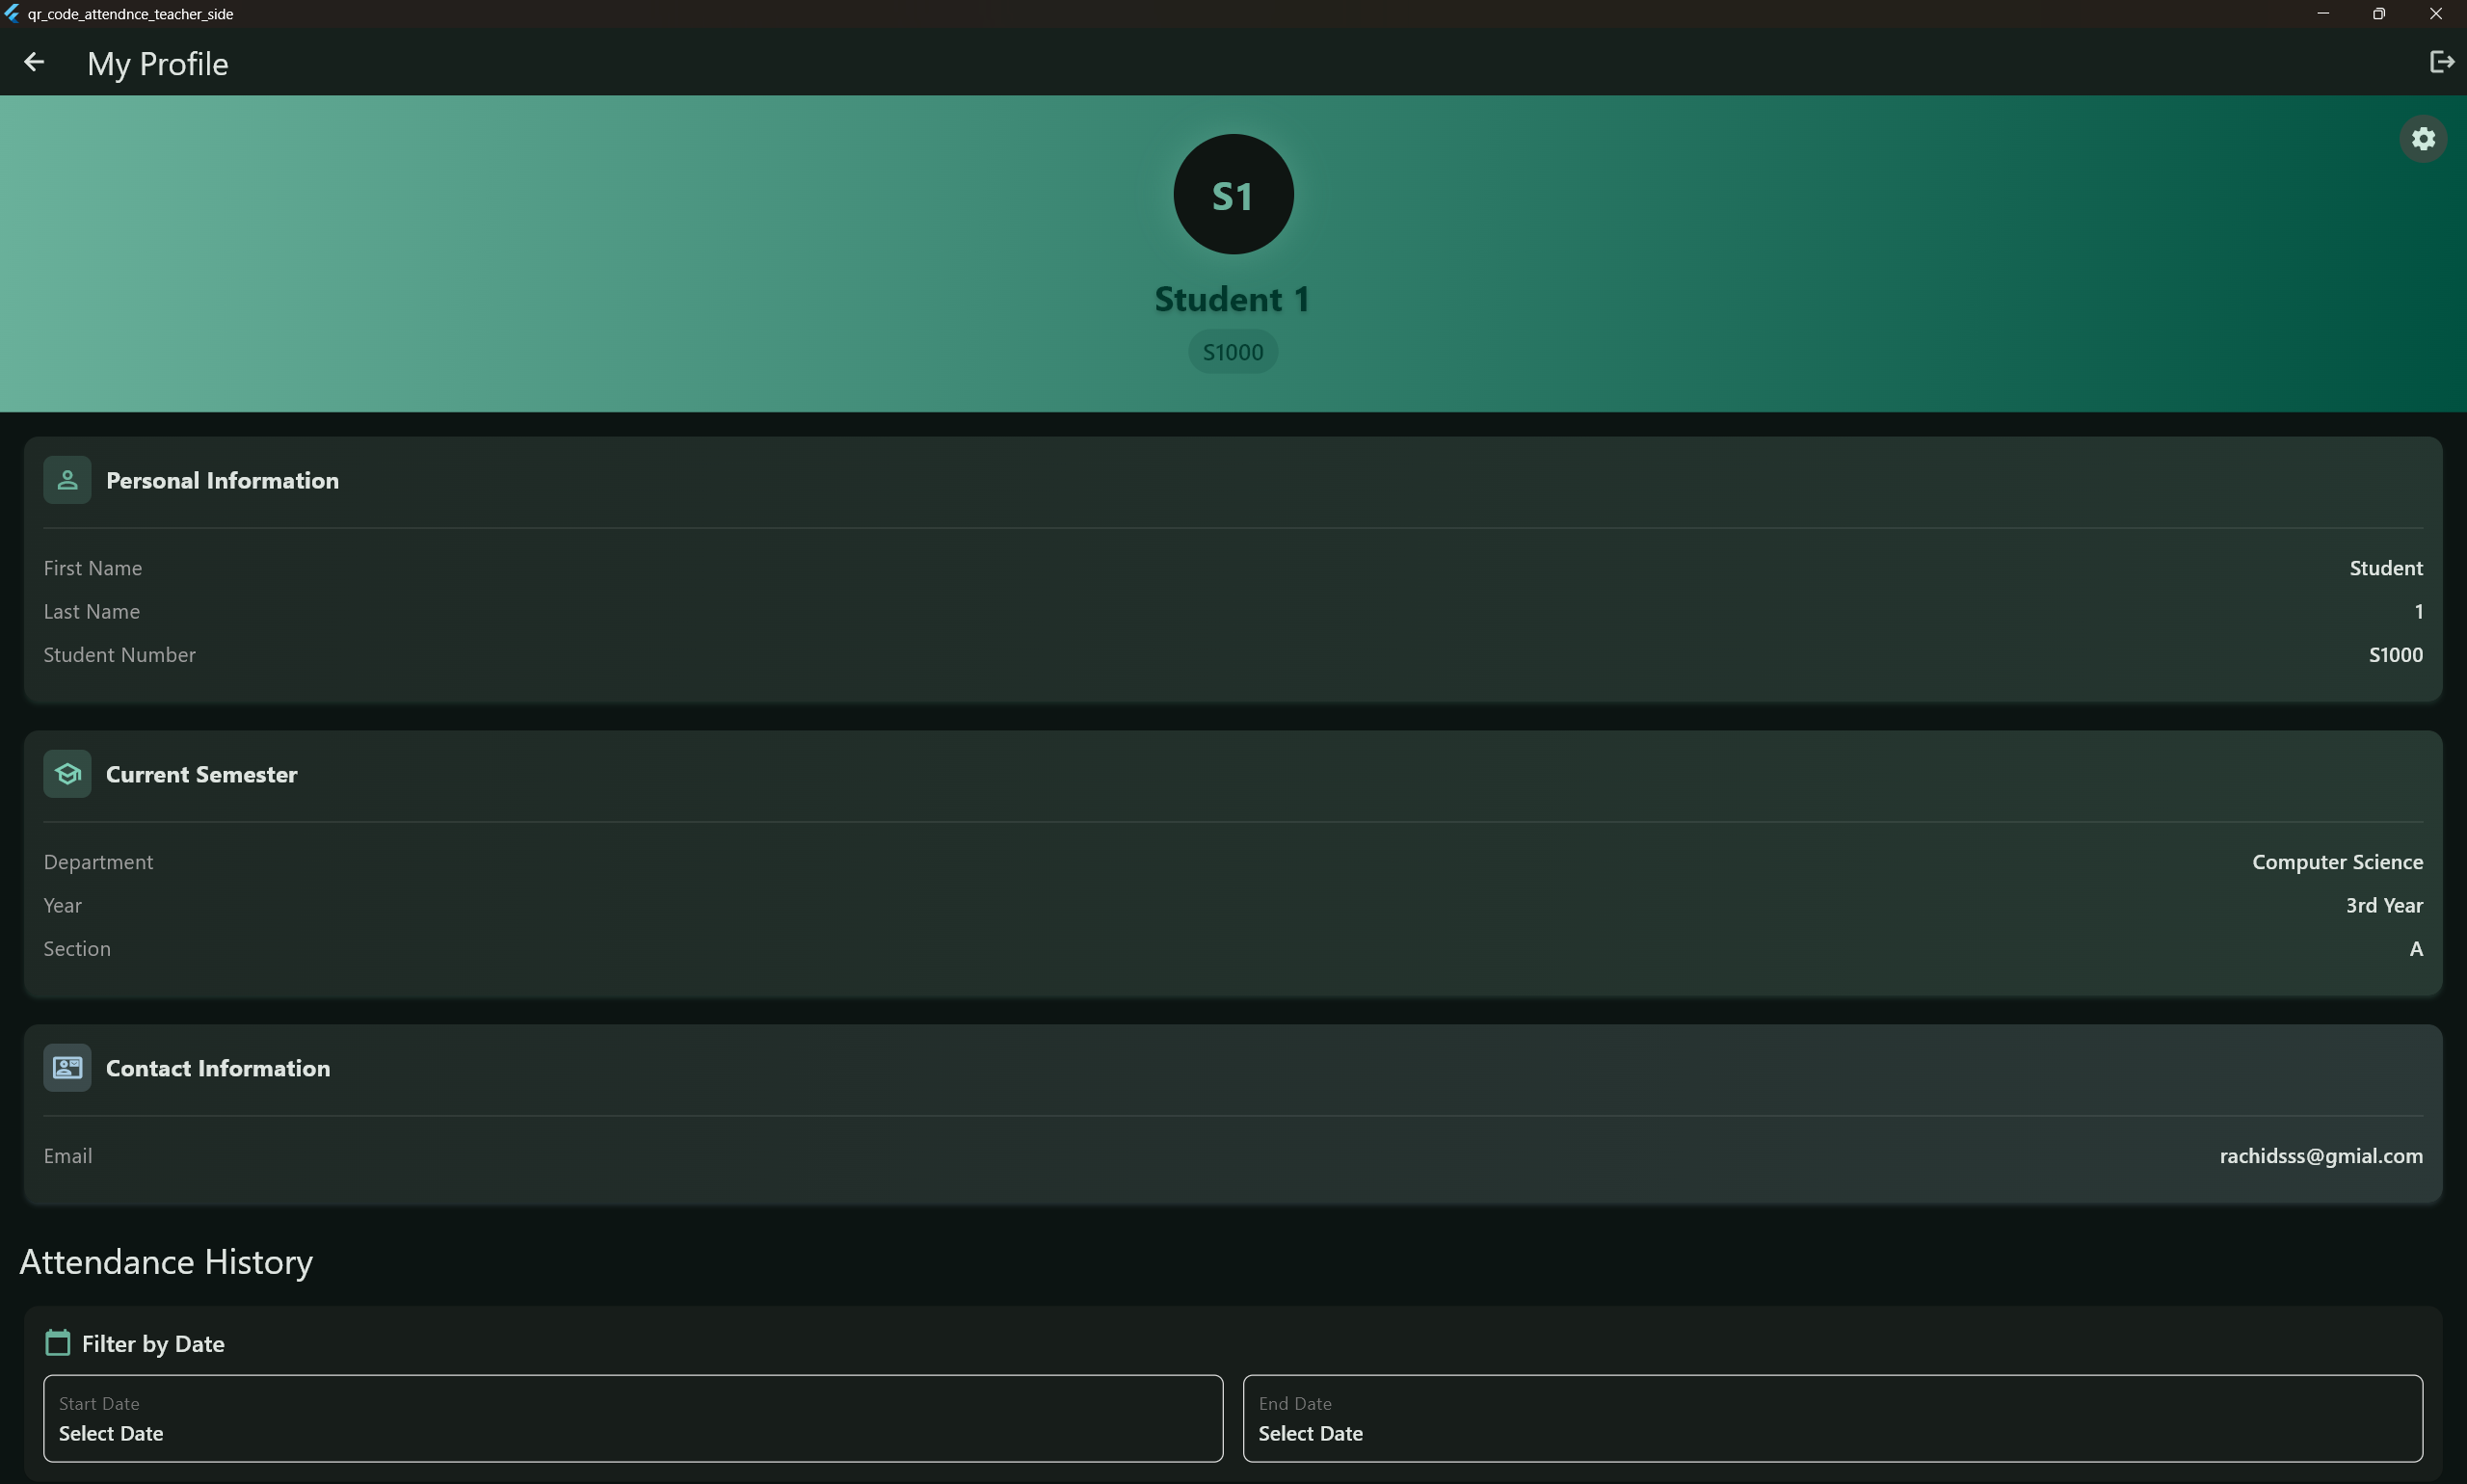
\includegraphics[width=0.45\textwidth]{images/rachid/teacher-side-studentpage-profileOfStudent-desktop.png}
    \caption{Detailed student profile view showing attendance history and academic information}
    \label{fig:student-profile}
\end{figure}

\needspace{4\baselineskip}
\subsection{Attendance Timeline}\nopagebreak[4]
\vspace{0.5cm}
\begin{figure}[H]
    \centering
    \begin{subfigure}[b]{0.35\textwidth}
        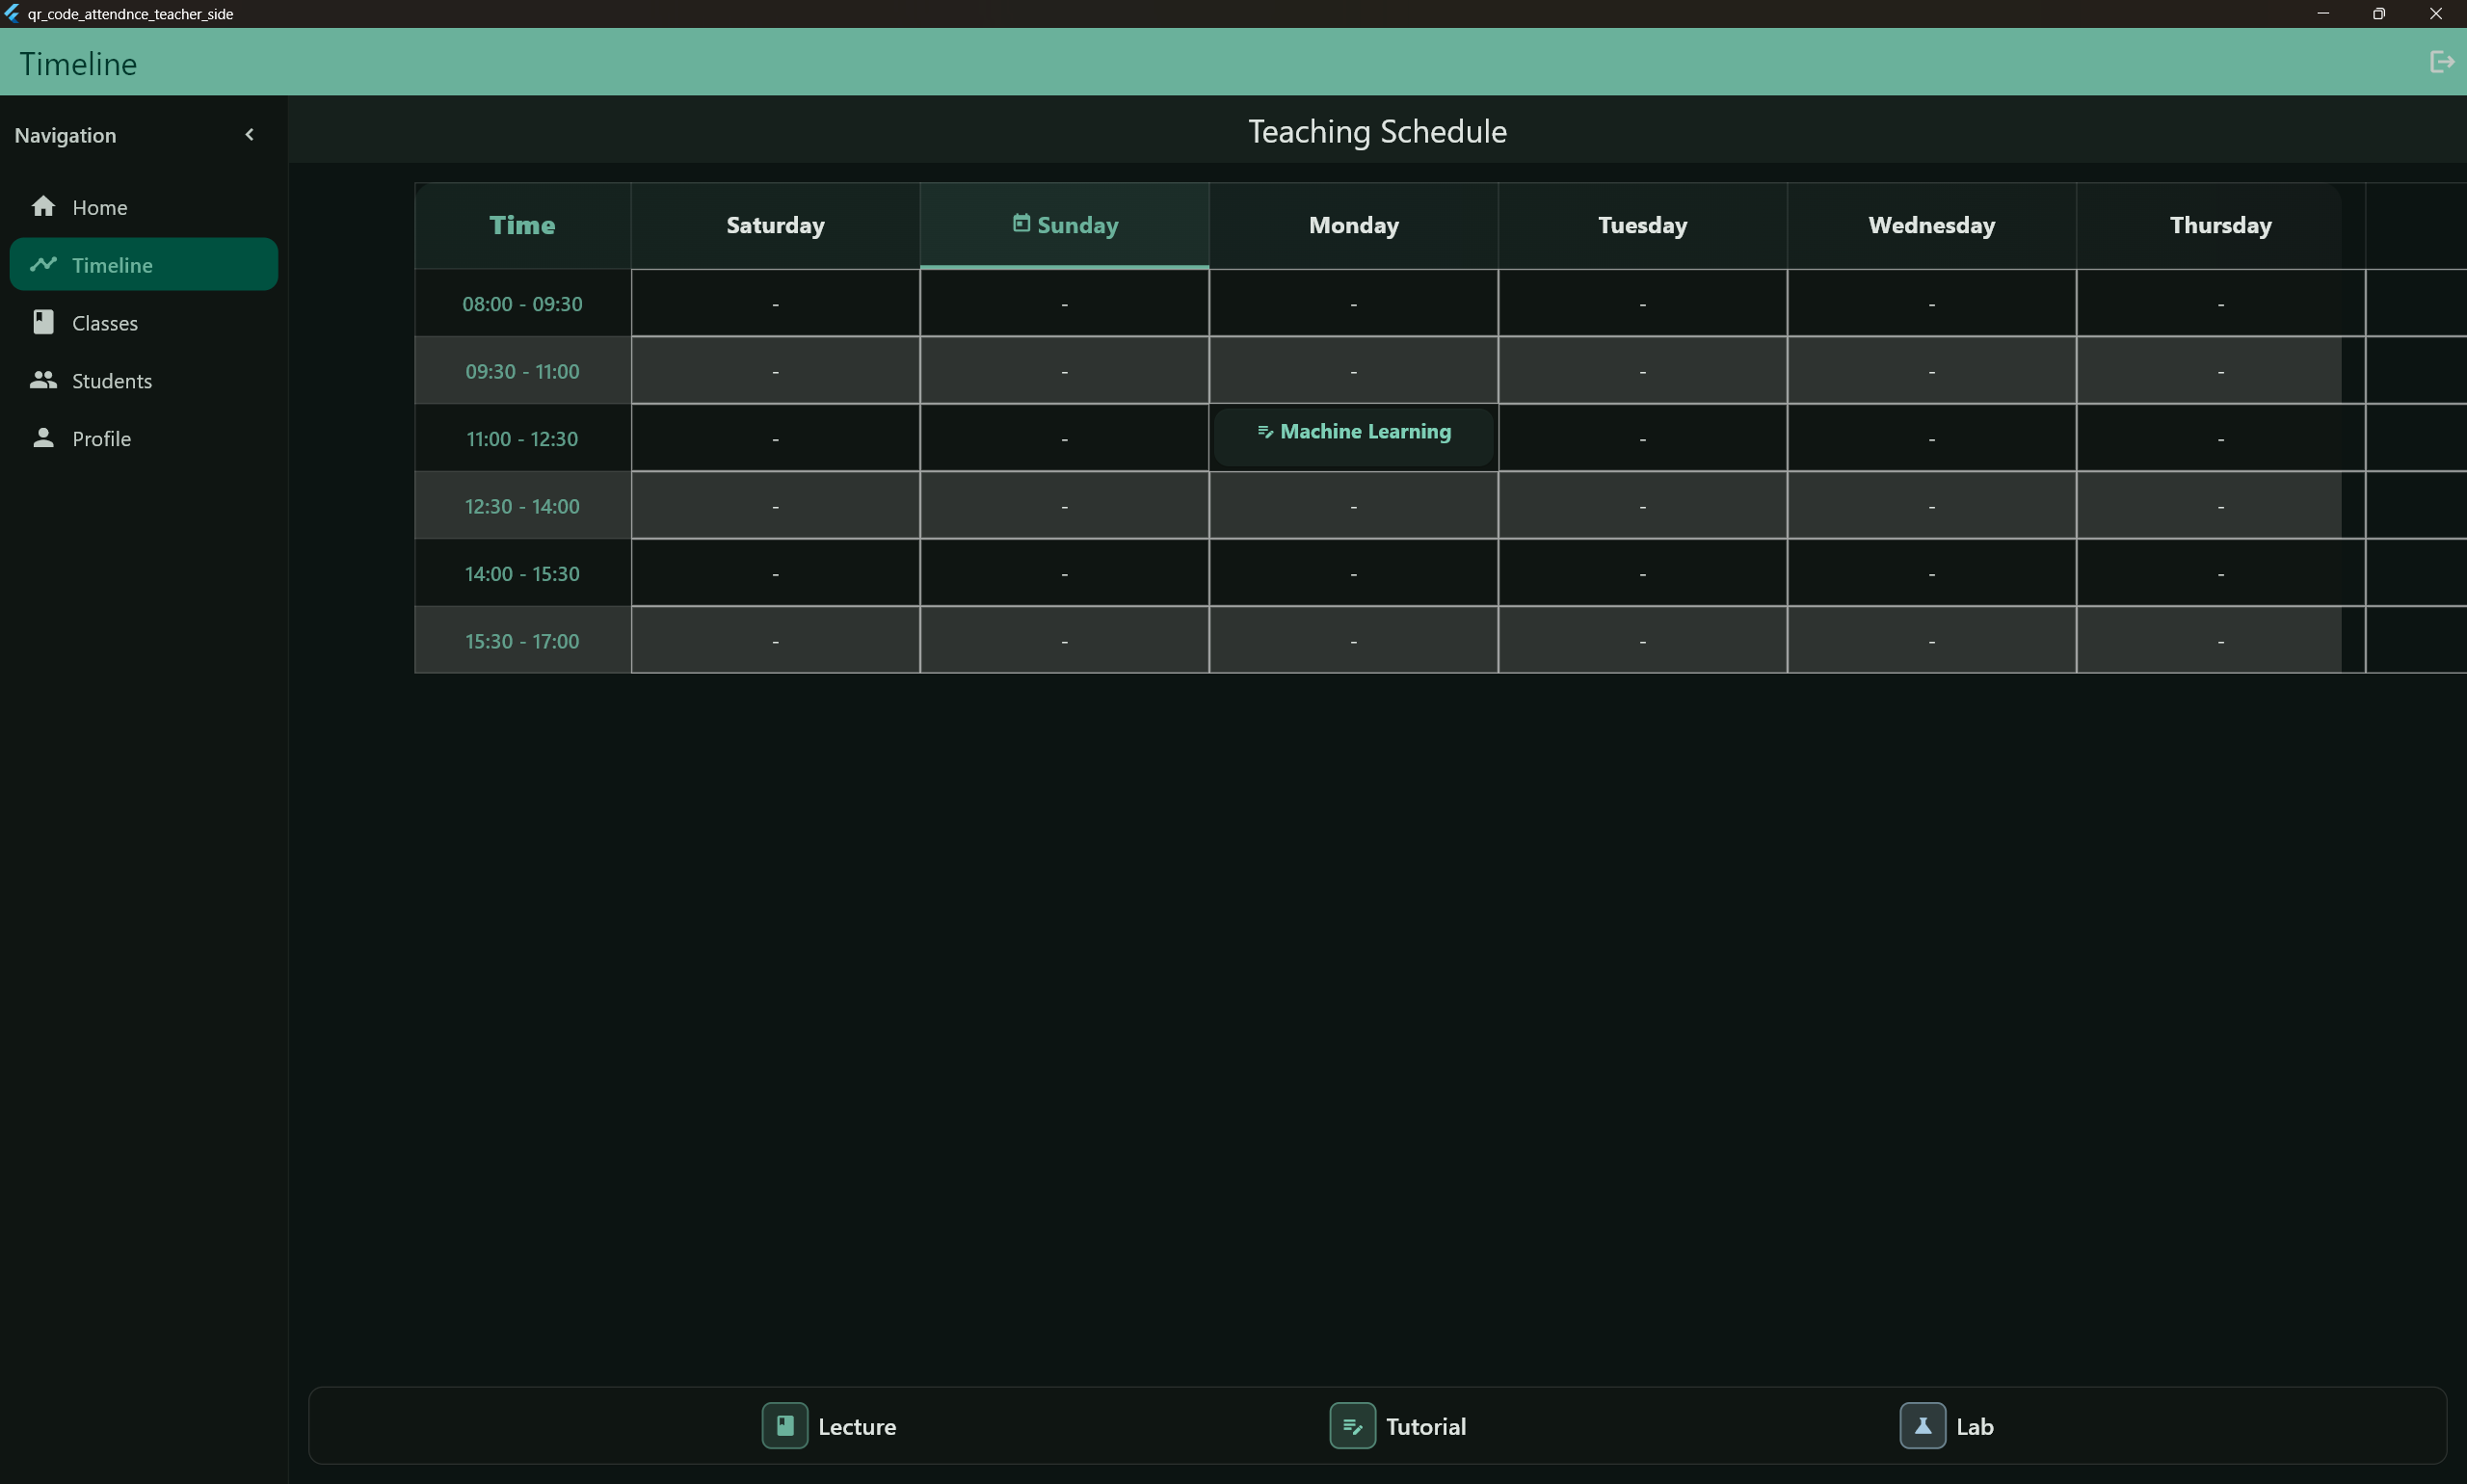
\includegraphics[width=\textwidth]{images/rachid/teacher-side-timeline.png}
        \caption{Mobile timeline view with chronological attendance events}
    \end{subfigure}
    \hfill
    \begin{subfigure}[b]{0.35\textwidth}
        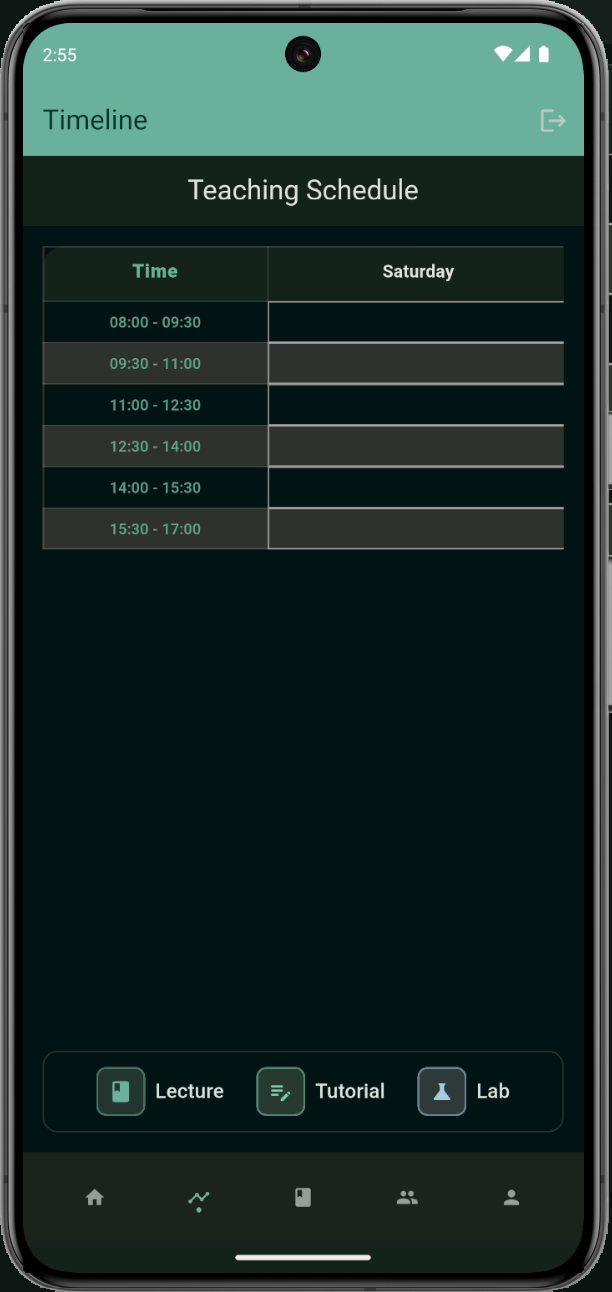
\includegraphics[width=\textwidth]{images/rachid/teacher-side-timeline-desktop.png}
        \caption{Desktop timeline with expanded event details and filtering options}
    \end{subfigure}
    \caption{Attendance Timeline Interface}
    \label{fig:timeline-interface}
\end{figure}

\needspace{4\baselineskip}
\subsection{Student Interface}\nopagebreak[4]
\vspace{0.5cm}
\begin{figure}[H]
    \centering
    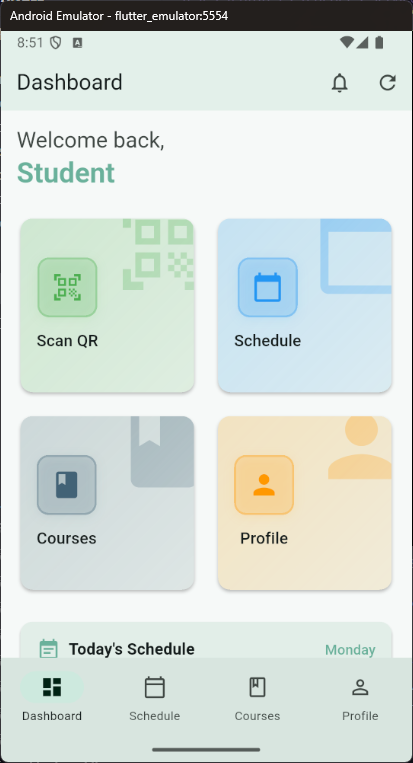
\includegraphics[width=0.45\textwidth]{images/rachid/student-side-homepage.png}
    \caption{Student Home Interface showing the main dashboard with quick access to courses and attendance information}
    \label{fig:student-home}
\end{figure}

\needspace{4\baselineskip}
\subsection{Student Course Management}\nopagebreak[4]
\vspace{0.5cm}
\begin{figure}[H]
    \centering
    \begin{subfigure}[b]{0.35\textwidth}
        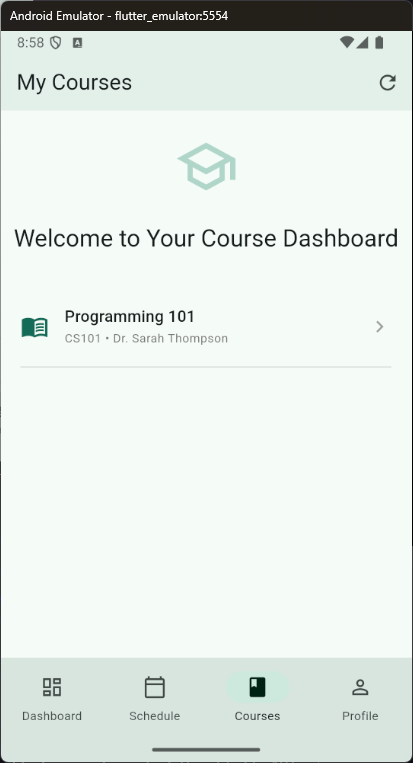
\includegraphics[width=\textwidth]{images/rachid/student-side-courses-home-1.png}
        \caption{Course overview dashboard showing enrolled courses}
    \end{subfigure}
    \hfill
    \begin{subfigure}[b]{0.35\textwidth}
        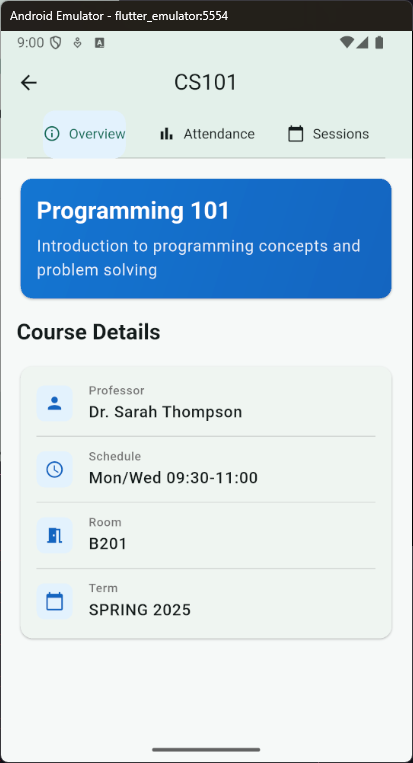
\includegraphics[width=\textwidth]{images/rachid/student-side-courses-home-classOverview-2.png}
        \caption{Detailed class overview with attendance statistics}
    \end{subfigure}
    \caption{Student Course Management Interface - Part 1}
    \label{fig:student-courses-1}
\end{figure}

\vspace{0.5cm}
\begin{figure}[H]
    \centering
    \begin{subfigure}[b]{0.35\textwidth}
        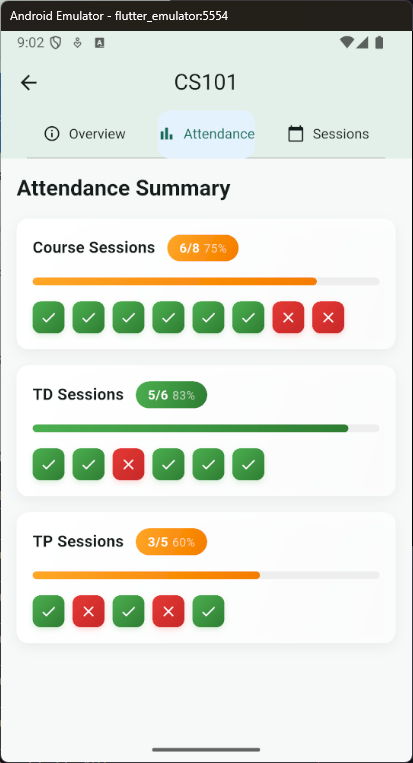
\includegraphics[width=\textwidth]{images/rachid/student-side-courses-home-classAttendance-3.png}
        \caption{Class attendance history and statistics}
    \end{subfigure}
    \hfill
    \begin{subfigure}[b]{0.35\textwidth}
        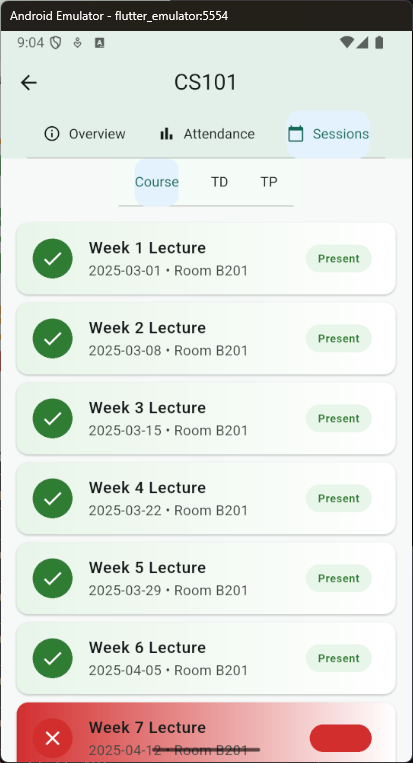
\includegraphics[width=\textwidth]{images/rachid/student-side-courses-home-classSessions-4.png}
        \caption{Session details and attendance records}
    \end{subfigure}
    \caption{Student Course Management Interface - Part 2}
    \label{fig:student-courses-2}
\end{figure}

\needspace{4\baselineskip}
\subsection{Student Timeline}\nopagebreak[4]
\vspace{0.5cm}
\begin{figure}[H]
    \centering
    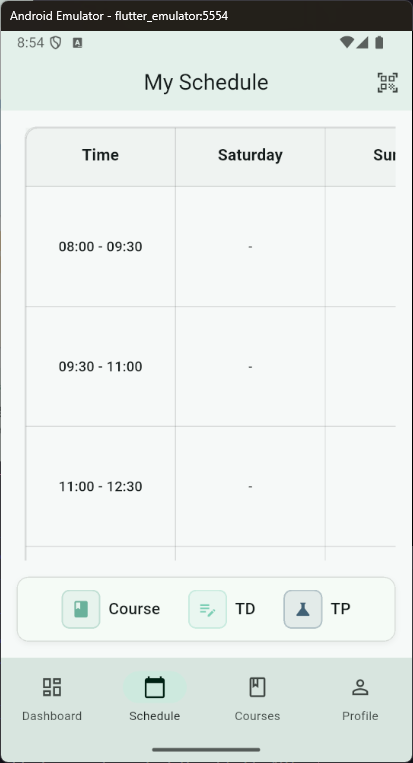
\includegraphics[width=0.45\textwidth]{images/rachid/student-side-timeline.png}
    \caption{Student Timeline Interface showing chronological view of attendance events and upcoming sessions}
    \label{fig:student-timeline}
\end{figure}
